
\section{Monotransit retrieval}
\label{sec:exp_monos}

As first real-world application, we consider the task of monotransit detection in a data set consisting of full-length light curves. For this experiment, 5000 LCSim light curves were generated, each of 27.4 days without missing data. 50\% of the light curves were injected with a single transit signal, and 50\% were left without signals. The task was to retrieve the transit signals by providing the correct transit time $t_0$, which was allowed to be any time within the duration of the transit.

The baseline method that we use for this task is based on \cite{foreman2016population}. In their work, a search algorithm similar to BLS is used to search for single transit events in Kepler data. In short, this algorithm fits a box function of given duration at each given point in time. The times at which the function is fitted are defined by the resolution of the search, e.g. one could choose a resolution of 0.25 times the trial duration. At each of these times, the depth of the box is varied until a best fit is found. Then the signal-to-noise ratio is calculated as $\text{SNR} = \delta/\sigma\cdot\sqrt{n} $, where $\delta$ is the depth of the signal, $\sigma$ the noise per time step and $n$ the number of data points the signal covers. The SNR is stored at each point where the function was fitted, so the result is an SNR time series, which is similar to the PTS. We will refer to the SNR time series as SNR-TS in the following. One adjustment that we made to the algorithm of \cite{foreman2016population}, is that instead of using a single trial duration of 0.6 days, we iterate over durations between 1 and 13 hours, with steps of 1 hour. For all these fits, we take the maximum over SNR's at each time step to define the SNR-TS. Subsequently, we identify peaks in the SNR-TS after standardization, i.e. subtracting its mean and dividing by its standard deviation. This is also different than the approach taken by \cite{foreman2016population}, as they compute the baseline of the SNR-TS with a running median filter, which is then subtracted from the SNR-TS prior to the search for peaks. However, we found that standardizing the SNR-TS allowed for better determination of detection thresholds. Before applying the algorithm, we detrend input light curves with a time-windowed median filter with a window of 12 hours. Altogether, we refer to this algorithm as Mono-BLS-12h.

Our method is based on the pre-trained RNN from previous sections. As shown in Figure \ref{fig:algorithm-mono_example}, a simple approach to detecting monotransit would be to consider each peak in the PTS above a certain threshold as a candidate. After a set of candidates has been collected this way, we give each candidate a score that is equal to their maximum PTS value. This maximum is used as indication of the network's certainty of a candidate relative to other candidates, and is thus used to set a threshold on which candidates are returned as detection.

To extend on this approach, we explore the use of the extra outputs $c_i$ at each time step $i$ that are given by the confidence network described in Section \ref{sec:extension_conf}. We use these values in two different ways, both with the aim of reducing the precision of the network detections. Figure \ref{fig:monos-conf_example} shows an example of the different ways $c$ is used in combination with the standard network output $y$, to define a new value, say $z$, which is used to set a detection threshold. \todo{test what results would be obtained for different peak thresholds with/without conf values, and with/without smoothing}

\begin{figure}
    \centering
    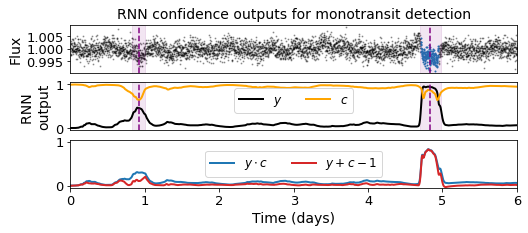
\includegraphics[width=0.65\linewidth]{Experiments/Figures/Monos/monos_example.png}
    \caption{\todo{caption}}
    \label{fig:monos-conf_example}
\end{figure}

Figure \ref{fig:monos-pr} shows the precision-recall curves for each method in the given task. From this figure, we observe that the RNN performed better than Mono-BLS-12h in this experiment. Moreover, no large differences were observed between the different RNN-based approaches. The use of an additional confidence parameter was therefore not of great influence on the results. Nevertheless, the fact that the RNN performed better overall than the box-fitting approach in this experiment, highlights the potential of our approach for this task. 

\begin{figure}
    \centering
    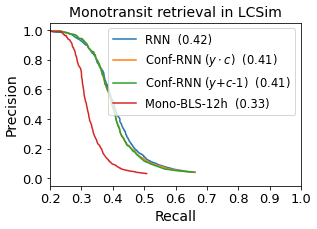
\includegraphics[width=0.4\linewidth]{Experiments/Figures/Monos/monos_pr.png}
    \caption{\todo{caption; between brackets shows area under the curve (AUC), also interpreted as average precision} \todo{explain that we have no uncertainties, and these results therefore only tell something about this specific experiment. future research should confirm these findings.}}
    \label{fig:monos-pr}
\end{figure}